Neste capítulo será detalhado o processo de desenvolvimento do framework Searchlight, e as ferramentas utilizadas para a construção do mesmo.

\section{Considerações Iniciais}
Durante  a fase de pesquisa deste projeto, descobriu-se uma variedade de recursos que poderiam ser usados na elaboração de um framework para visualização de mapas. Muitos destes recursos já estavam no cronograma do projeto, outros foram adicionados  e alguns ficaram fora do cronograma e colocados na lista de trabalhos futuros.

Inicialmente a meta do framework era apenas encontrar uma maneira de visualizar mapas de crowdsourcing de forma mais limpa e sucinta através de técnicas de agrupamento aliadas a hierarquia de zoom. Mas no decorrer das pesquisas percebeu-se que seria interessante adicionar alguns recursos como filtro por categoria e foco em grupo. 

Também foi adicionado ao projeto a possibilidade de gerar e compartilhar um mapa web sem precisar escrever uma linha de código.
O único requisito é fornecer um endereço web onde o gerador de mapas deve buscar os dados geográficos do mapa. Neste caso, o usuário não precisa mais saber programar para poder usufruir dos recursos do framework e a única preocupação dele fica depositada sobre o conteúdo do mapa.

Em relação ao conteúdo usado pelo compartilhador de mapas, o framework atualmente suporta o armazenamento numa planilha eletrônica ou em um arquivo de formato JSON\footnote{Formato muito usado para troca de dados entre websites \url{http://www.json.org}}. Quando o conteúdo é oriundo de planilha eletrônica é necessário que esta esteja armazenada no Google Docs e seja pública. De forma similar, quando o conteúdo é armazenado em um arquivo JSON é necessário que o website que hospeda o arquivo suporte o protocolo JSONP. Caso contrário, o usuário deve instalar o framework Searchlight no website que deseja visualizar o mapa.


Em relação as ferramentas que foram utilizadas no projeto, o objetivo inicial era usar a api do Google Maps para a visualização dos mapas. Porém,  na época em que esta pesquisa era feita, circulava notícias que o Google estaria mudando seus termos de serviço e iria começar a cobrar\footnote{Uma notícia sobre o inicio das cobranças do Google Maps \url{http://goo.gl/f1E3K}} pelo uso da API do Google Maps. Além disso, no mesmo período, a Apple anunciou que iria abandonar o uso do Google Maps em seus smartphones e adotaria uma solução própria. Isto trouxe a necessidade de procurar uma alternativa ao Google Maps, e a alternativa encontrada foi a biblioteca open-source \textbf{Leaflet.js} que será descrita no decorrer deste capítulo.




\section{Ferramentas e bibliotecas us	tilizadas}

Um framework, em desenvolvimento de software, é uma abstração que une códigos comuns entre vários projetos de software provendo uma funcionalidade genérica. Um framework pode atingir uma funcionalidade específica, por configuração, durante a programação de uma aplicação. Ao contrário das bibliotecas, é o framework quem dita o fluxo de controle da aplicação, chamado de Inversão de Controle\footnote{Definição completa em: \url{http://pt.wikipedia.org/wiki/Framework}}.

De modo geral, um framework é conjunto de ferramentas que trabalham em conjunto. O que une as ferramentas são as regras do framework que tem como objetivo prover as funcionalidades que motivaram a criação do framework.

O framework Searchlight tem como objetivo facilitar a criação e a visualização de mapas de crowdsourcing por meio de automatização do processo de criação do mapa. O público alvo abrange tanto  programadores de mapas web quanto  usuários sem nenhum conhecimento de programação. Para atingir este objetivo o framework faz uso do seguinte conjunto de ferramentas: GitHub, Lealflet.js, jQuery, Tabletop.js e RapydScript. 

\subsection{Github}
	
\subsection{GithubPages}

\subsection{Aplicações Comerciais de Agrupamento de Pontos}
		Durante a fase de pesquisa, deste trabalho, foi feito uma busca por aplicações acadêmicas, e comerciais, que já fizessem o uso de algorítimos de agrupamento de pontos. Duas aplicações se destacaram: MarkerClusterer e Leaflet.MarkerCluster.
		\subsubsection{MarkerClusterer}
		
		MarkerClusterer \cite[188]{livroGoogleApiV3} é uma ferramenta fornecida pelo google que estende o uso da API do Google Maps para o uso de algorítimos de agrupamentos.
		
		MarkerClusterer é uma solução baseada em grelha. Ela agrupa marcadores de acordo com sua distância ao centro de um grupo. Quando um marcador é adicionado, ele pesquisa sua posição em todos os grupos. Caso não seja colocado em nenhum grupo, um novo grupo é criado para este marcador. A \autoref{fig-markerclusterer} demonstra a aplicação da ferramenta nos marcadores de um mapa.
	\begin{figure}[htb]
	\caption{\label{fig-markerclusterer}Exemplo de utilização da API MarkerClusterer }
	\begin{center}
	    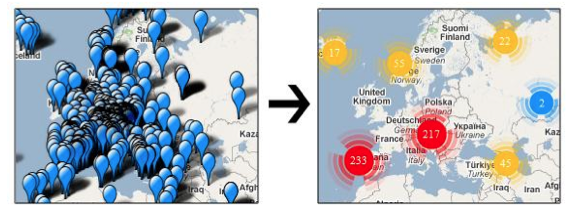
\includegraphics[scale=0.8]{markerclusterer}
	\end{center}
		\legend{Fonte: \cite[figura 20]{silva2010solap+}  }
\end{figure}

		\subsubsection{Leaflet.MarkerCluster}
		Assim como a biblioteca MarkerCLusterer estende a API do Google Maps para uso de agrupamento de marcadores, o plugin Leaflet.MarkerCluster serve como uma extensão para a API, de visualização de mapas, Leaflet.js\footnote{\url{http://leafletjs.com} é uma alternativa  a API do Google Maps, pois fornece um melhor suporte a dispositivos móveis como tablets e smartphones }. 
		
		Este plugin, faz basicamente as mesmas funções da ferramenta MarkerCluster, porém com algumas melhorias. Por exemplo, ao fazer zoom o mapa exibe uma pequena animação do processo de agrupamento; ao se passar o mouse sobre um marcador do grupo o mapa exibe um polígono que mostra os limites alcançados pelo grupo; os grupos que não são visíveis  na visualização atual do mapa são retirados do mapa para aumentar a performance. Além dessas melhorias, uma que merece destaque é a sua incrível capacidade de customização. 

		Ao contrário da biblioteca MarkerClusterer, o plugin Leaflet.MarkerCluster possui um documentação bem completa que pode ser encontrada em \citeonline{gitleafletmaker}. Inicialmente, procurou-se por uma documentação mais abrangente da biblioteca MarkerCluster, mas até o momento da confeção desse trabalho não foi possível encontrar nada além de alguns poucos exemplos de uso. Isto, e outros fatores, contribuíram para a escolha da biblioteca Leaflet.js como API de visualização de mapas do framework Searchlight.
		  
\subsection{Leaflet.js}
\subsection{Leaflet.markercluster}
\subsection{Leaflet.spin}

\subsection{jQuery}
\subsection{jQueryUI}

\subsection{TableTop.js}

\subsection{Rapydscript}


\section{Arquitetura do Sistema}
\subsection{Processamento de dados}
\subsection{Interface com usuário} 
\subsection{Compartilhamento de mapas}
s